\documentclass{article}
\usepackage{graphicx}
\usepackage{float}
\usepackage{subcaption}
\usepackage{amsmath}
\graphicspath{{images/}}
\usepackage{caption}
\captionsetup[figure]{position = below,}
\usepackage{listings}
\usepackage{xcolor}
\DeclareCaptionFont{white}{\color{white}}
\DeclareCaptionFormat{listing}{%
  \parbox{\textwidth}{\colorbox{gray}{\parbox{\textwidth}{#1#2#3}}\vskip-4pt}}
\captionsetup[lstlisting]{format=listing,labelfont=white,textfont=white}
\lstset{frame=lrb,xleftmargin=\fboxsep,xrightmargin=-\fboxsep, columns=fullflexible}


\title{Finding the galvanometer current from a Wheatstone Bridge Network of conductors, by solving numerically a system of equations}

\author{Indranil Ghosh\\Jadavpur University\\Physics department\\indranilg49@gmail.com}
\date{\today}
\begin{document}
\maketitle
\section{Abstract}
This project is a simple application of Numerical method to solve the values of currents from a system of equations for the Wheatstone's bridge network of conductors. Methods used: Kirchoff's laws for steady currents, Maxwell's cyclic currents and Gauss-Jordan method to solve the system of equations. Programming language used: Python and packages used: Numpy and Pandas. 

\section{Introduction}
Invented by Samuel Hunter Christie in 1833 and improved and popularised by Sir Charles Wheatstone in 1843, the Wheatstone bridge network of four resistances is one of the most commonly used methods for comparing resistances and is for use with currents of zero frequency. The Wheatstone's bridge is a fundamental bridge and is used in accurate measurements, but can be further modified into Kelvin Bridge, Carey Foster Bridge, Maxwell's bridge, etc.

\section{Kirchoff's Laws}
\subsection{Kirchoff's Current Law(KCL)}
Also known as Kirchoff's First Law, it states: \textit{The algebraic sum of currents in a network of conductors meeting at a point is zero}. \\
\begin{center}
1.$\sum_{k=1}^n I_k=0$
2.$\sum_{k=1}^n I^*_k=0$ [complex currents]
\end{center}
This law is based  on the conservation of charge.
\subsection{Kirchoff's Voltage Law(KVL)}
Also known as Kirchoff's Second Law, it states: \textit{The algebraic sum of the emfs in any closed circuit or loop is equal to the algebraic sum of the products of the resistances of each link of the circuit or loop and the currents of zero frequency flowing through them, provided Ohm's Law is obeyed for each link}
\begin{center}
1.$\sum_{k=1}^n V_k=0$\\
2.$\sum_{k=1}^n V^*_k=0$ [complex voltage]
\end{center}
This law is based on the conservation of energy
\section{Maxwell's cyclic currents}
Maxwell imagined that a specified cyclic current flows in each loop and considered all clockwise currents as positive. The current in any branch is thus the algebraic difference between the cyclic currents in the loop it separates.

\section{Gauss-Jordan Algorithm}
This algorithm reduces a given system of equations $AX=B$ to a diagonal system of equations $IX=D$, where \textbf{I} is the identity matrix. This uses elimentary row operations to transform the augmented matrix $[A \vert B]$ to \textbf{Reduced Row Echelon Form (RREF)}. The reduced system gives the solution vector \textbf{X}.

\section{Problem}
\begin{figure}[H]
\centering 
\noindent\makebox[\textwidth]{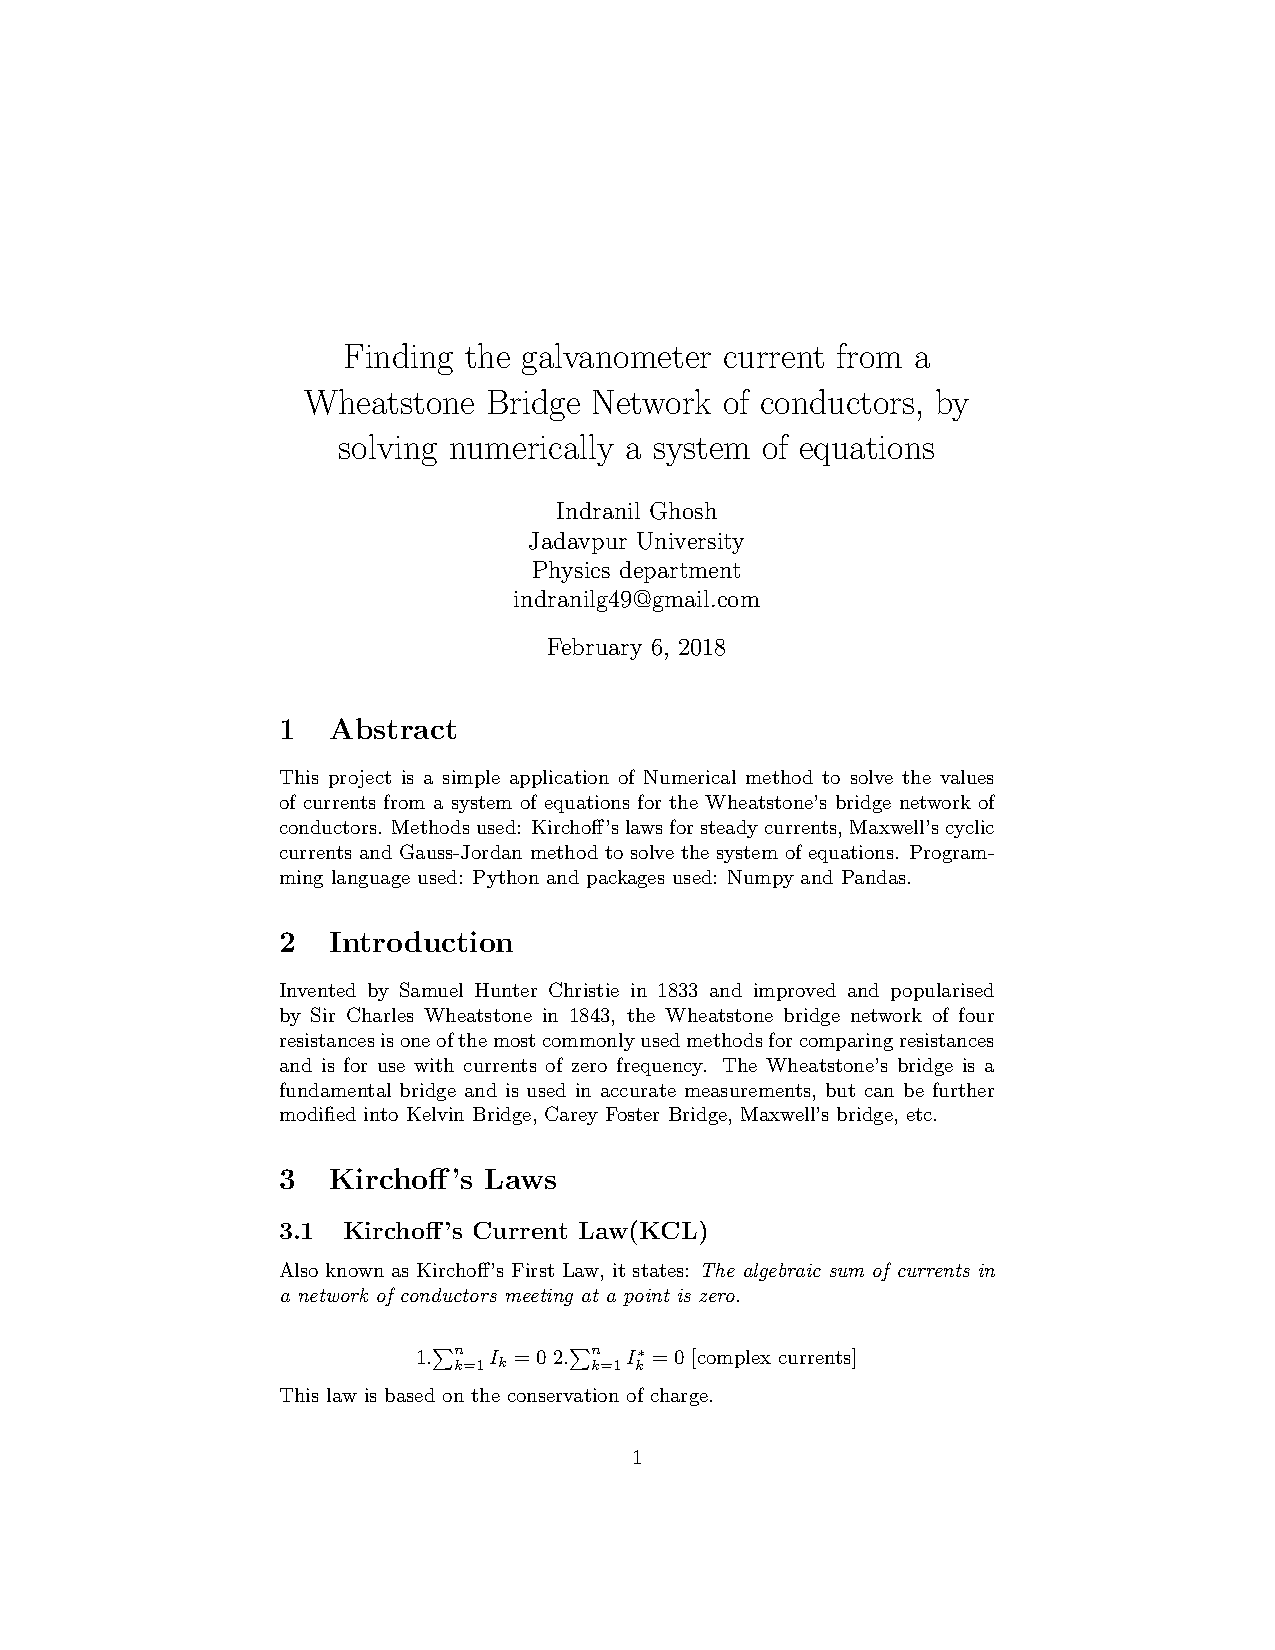
\includegraphics[scale=0.4 ]{wheatstone}}%
\caption{Wheatstone Bridge Network}
\end{figure}
here the cyclic currents are $I_1, I_2$ and $I_3$. R includes the resistance of the cell of emf E, that supplies current to the bridge. $R_g$ is the resistance of the galvanometer. Our goal is to calculate the currents $I, I_1, I_2$ and $I_g$. We also calculate $V_g$, the voltage of the node B, relative to D. \\
\\
The equations of the bridge, applying Kirchoff's Laws and Maxwell's cyclic currents, are:
\begin{equation}
IR+(I-I_1)R_3+(I-I_1+I_g)R_4-I_gR_g=E 
\end{equation}
\begin{equation}
I_1R_1+I_gR_g-(I-I_1)R_3=0 
\end{equation}
\begin{equation}
(I_1-I_g)R_2-(I-I_1+I_g)R_4-I_gR_g=0
\end{equation}
We know $I_g=I_1-I_2$.  Substituting this relation in the above equations and rearrenging them, we get,
\begin{equation}
(R+R_3+R_4)I-R_3I_1-R_4I_2=E
\end{equation}
\begin{equation}
-R_3I+(R_1+R_g+R_3)I_1-R_gI_2=0
\end{equation}
\begin{equation}
-R_4I-R_gI_1+(R_g+R_2+R_4)I_2=0
\end{equation}

We write this system of equations in Matrix form: \\
\begin{equation}
\begin{bmatrix}
R+R_3+R_4 & -R_3 & -R_4 \\
-R_3 & R_1+R_g+R_3 & -R_g \\
-R_4 & -R_g & R_g+R_4
\end{bmatrix}
\begin{bmatrix}
I \\
I_1 \\
I_2
\end{bmatrix}
=
\begin{bmatrix}
E \\
0 \\
0
\end{bmatrix}
\end{equation}
We solve this using Gauss-Jordan algorithm and extract the values of $I_1, I_2$ and $I_3$. From this values we calculate $I_g=I_1-I_2$ and $V_g=({R_1 \over{R_1+R_2}}-{R_3 \over{R_3+R_4}})E$.

\section{Python Code}
\begin{lstlisting}[language=Python, frame=single]
import numpy as np
import pandas as pd

def GJ(A, b): # Gauss-Jordan Algorithm
      Aug=np.concatenate((A, b), axis=1)
      row=len(A)
      col=len(A[0])
      for i in range(col-1):
              m=Aug[i, i]
              k=i
              for R in range(i, row):
                  if Aug[R, i]>m:
                          m = Aug[R, i]
                          k = R
              t=np.copy(Aug[i,])
              Aug[i,]=Aug[k,]
              Aug[k,]=t
              for j in range(i+1,row):
                      s=Aug[j,i]/Aug[i, i]
                      Aug[j,]-=Aug[i,]*s
      for i in range(row): Aug[i,]/=Aug[i, i]
      d=1
      for r in range(row-2,-1,-1):
              for k in range(r, -1, -1):
                      Aug[k,]=Aug[k,]-Aug[k, k+d]*Aug[k+d]
              d+=1
      return(Aug.T[row:].T)

def Solve_bridge(R, R1, R2, R3, R4, Rg, E):
        A=np.array(([R+R3+R4, -R3, -R4],
                    [-R3, R1+Rg+R3, -Rg], [-R4, -Rg, Rg+R2+R4]))
        B=np.array(([E], [0.], [0.]))
        X=GJ(A, B)
        I=X.item(0)
        I1=X.item(1)
        I2=X.item(2)
        Ig=I1-I2
        Vg=(R1/(R1+R2)-R3/(R3+R4))*E
        D=pd.DataFrame({'parameters':['I', 'I1', 'I2', 'Ig', 'Vg'],
                        'values':[I, I1, I2, Ig, Vg]})
        D=D.set_index('parameters')
        return D

print (Solve_bridge(0, 100., 10., 1000., 100.01, 10., 2.)) #Example
\end{lstlisting}
\begin{thebibliography}{9}
\bibitem{knuthwebsite}
\texttt{Numerical Methods by Jain, Iyengar}
\bibitem{knuthwebsite}
\texttt{Electricity and Magnetism, C.J. Smith}
\bibitem{knuthwebsite}
\texttt{Wikipedia,Wheatstone bridge, https://en.wikipedia.org/wiki/Wheatstone bridge}
\bibitem{knuthwebsite}
\texttt{Wikipedia, Kirchoff's circuit Laws, https://en.wikipedia.org/wiki/Kirchhoff's circuit laws}
\end{thebibliography}
\end{document}
\end{document}